\documentclass{article}
\usepackage{graphicx} 
\usepackage{booktabs}
\usepackage{array}
\usepackage{amsmath}
\usepackage{subcaption}

\graphicspath{{figures/}} % assumes all images are stored in figures/ folder

\title{Debris Field Loading during Tsunami Events}
\date{September 2025}

\begin{document}

\maketitle

\section{Introduction}
\begin{itemize}
    \item Tsunami-driven debris fields impose both \textbf{short-duration impact loads} and \textbf{sustained damming loads} on coastal infrastructure.
    \item Predicting these forces is challenging because they depend on highly nonlinear fluid–structure–debris interactions.
    \item Debris characteristics that influence loading include:
    \begin{itemize}
        \item Orientation (longitudinal, transverse, random).
        \item Size distribution (single-size vs multi-size).
        \item \textbf{Surface area density} (ratio of debris area to water surface area).
    \end{itemize}
    \item This study investigates debris loading mechanisms through large-scale flume experiments, focusing on how debris configuration and surface area density influence impact and damming forces.
\end{itemize}

\section{Testing Methodology}
\begin{itemize}
    \item Experiments were conducted in a tsunami flume equipped with a rigid mid-flume structure.
    \item Two wave types were tested: \textbf{unbroken solitary waves} (primary focus) and \textbf{broken solitary waves} (discarded in this summary due to negligible forces).
    \item Debris fields were generated in three configurations:
    \begin{itemize}
        \item Regular longitudinal (aligned with flow).
        \item Regular transverse (perpendicular to flow).
        \item Random (both single-size and multi-size).
    \end{itemize}
    \item Force records were decomposed using Butterworth filters:
    \begin{itemize}
        \item \textbf{High-pass} filtering to isolate short-duration impact peaks.
        \item \textbf{Low-pass} filtering to capture long-duration damming forces.
    \end{itemize}
\end{itemize}

\begin{figure}[htbp]
    \centering
    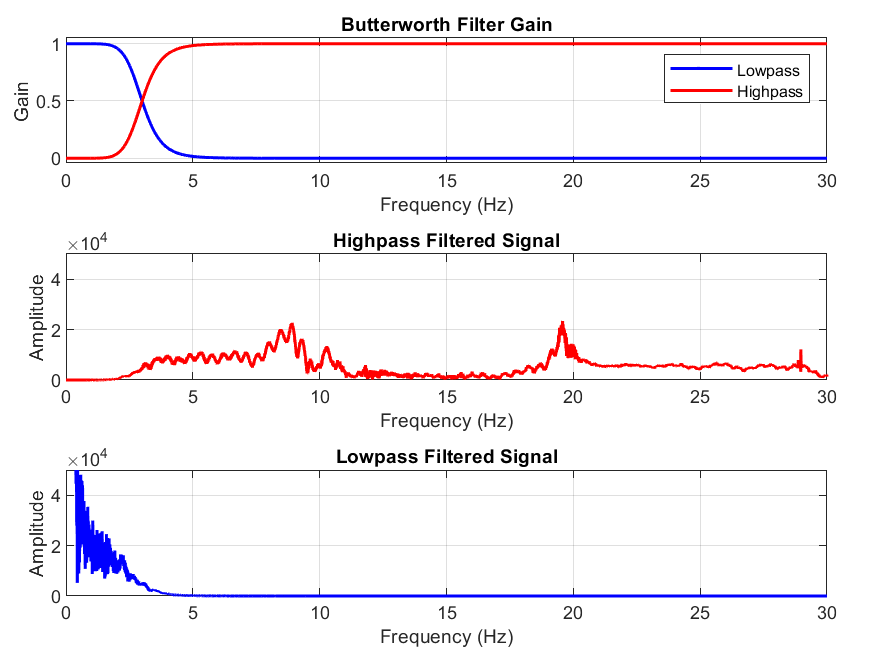
\includegraphics[width=0.8\textwidth]{high_low_pass.png}
    \caption{Force decomposition via Butterworth filters. High-pass isolates impact peaks; low-pass extracts damming loads.}
    \label{fig:high_low_pass}
\end{figure}

\section{Peak Force Identification}
\begin{itemize}
    \item Video evidence and filtered signals revealed that debris impact occurs in two distinct stages:
    \begin{itemize}
        \item \textbf{First impact}: initial contact with the unsubmerged portion of the structure.
        \item \textbf{Later impacts}: delayed, submerged strikes driven by overtopping, suction, and debris recirculation.
    \end{itemize}
    \item This staged behavior was consistent across debris types and configurations, highlighting the importance of distinguishing between early and late peaks.
\end{itemize}

\begin{figure}[htbp]
    \centering
    \begin{subfigure}{0.48\textwidth}
        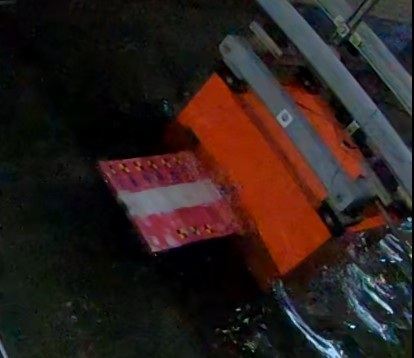
\includegraphics[width=\linewidth]{first_impact.jpg}
        \caption{Initial unsubmerged debris strike.}
    \end{subfigure}
    \hfill
    \begin{subfigure}{0.48\textwidth}
        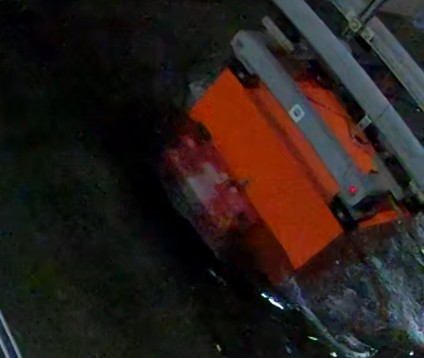
\includegraphics[width=\linewidth]{second_impact.jpg}
        \caption{Later submerged strike caused by overtopping/suction.}
    \end{subfigure}
    \caption{Sequential debris impact stages observed in video recordings.}
    \label{fig:video_impacts}
\end{figure}

\section{Results: Impact Forces (Unbroken Waves)}

\subsection{Regular Configurations}
\begin{itemize}
    \item \textbf{First impact peaks} increased almost linearly with the number of debris elements, reflecting simultaneous group impacts when debris aligned with the structure.
    \item \textbf{Later impacts} exhibited nonlinear growth, saturating at higher debris counts due to hydrodynamic cushioning and interference effects.
    \item Longitudinal layouts produced the highest impact forces, while transverse layouts yielded smaller peaks due to water cushioning between debris and the structure.
    \item The role of \textbf{surface area density} is critical:
    \begin{itemize}
        \item At equal density, larger debris groups were more spread out across the flume width.
        \item For example, 24 pieces at the same density as 8 pieces occupied a greater span than the structure, reducing the probability that all would strike simultaneously.
    \end{itemize}
    \item For the \textbf{24T and 16T2 tests}, the surface area of the debris field exceeded that of the structure.
    \begin{itemize}
        \item Video analysis confirmed that only part of the debris actually contacted the structure.
        \item The force data for these trials was therefore \textbf{remapped and corrected} to reflect the effective impact area rather than nominal debris count.
    \end{itemize}
\end{itemize}

\begin{figure}[htbp]
    \centering
    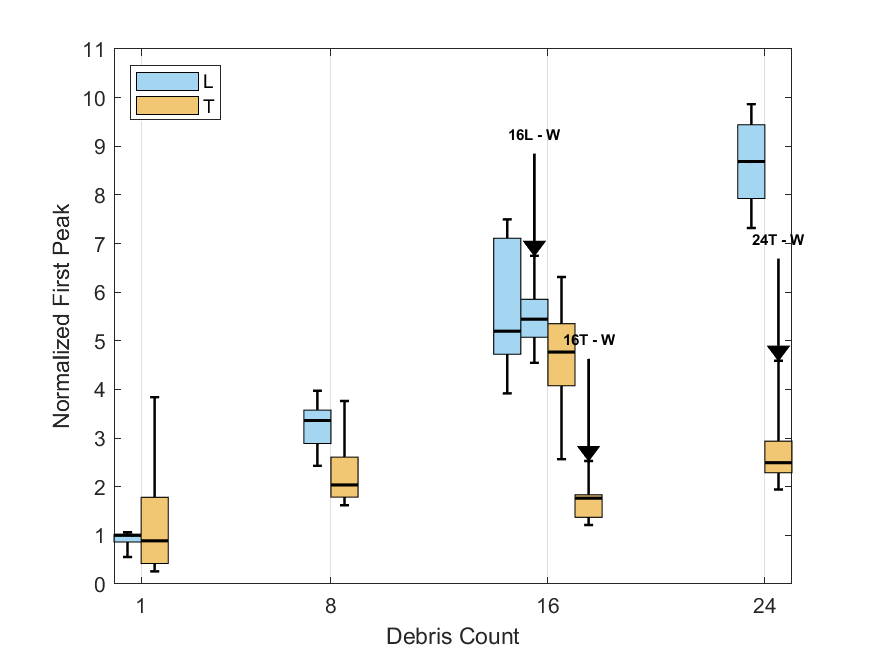
\includegraphics[width=0.8\textwidth]{FirstPeak_Regular_SplitByTrial.png}
    \caption{First peak forces in regular arrangements (split by trial). Nearly linear scaling with debris count observed.}
    \label{fig:firstpeak_regular_split}
\end{figure}

\begin{figure}[htbp]
    \centering
    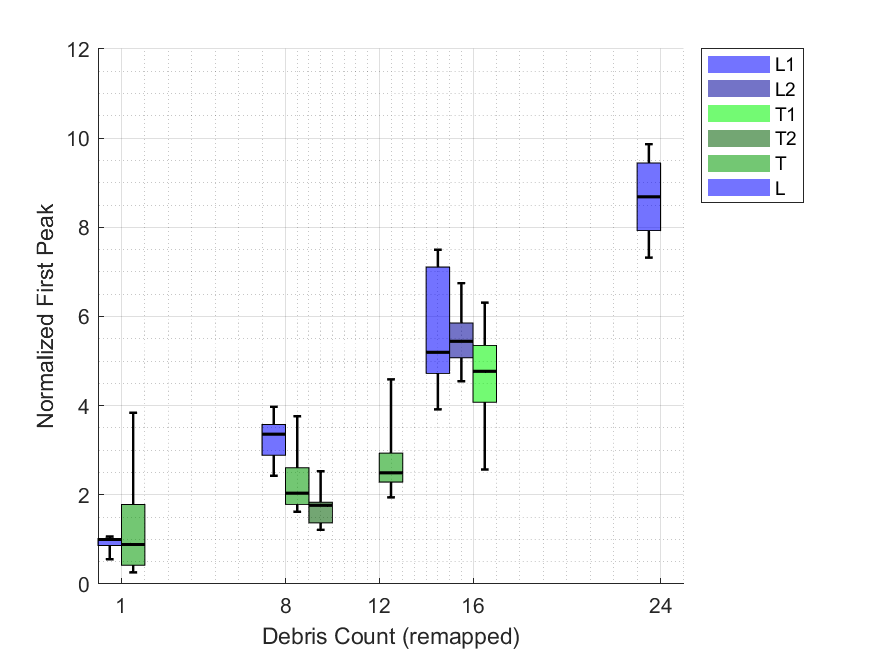
\includegraphics[width=0.8\textwidth]{FirstPeak_Regular_RemappedT.png}
    \caption{First peak forces in regular arrangements (remapped to normalized time). Includes corrected data for 24T and 16T2 trials where debris exceeded structure area.}
    \label{fig:firstpeak_regular_remap}
\end{figure}

\begin{figure}[htbp]
    \centering
    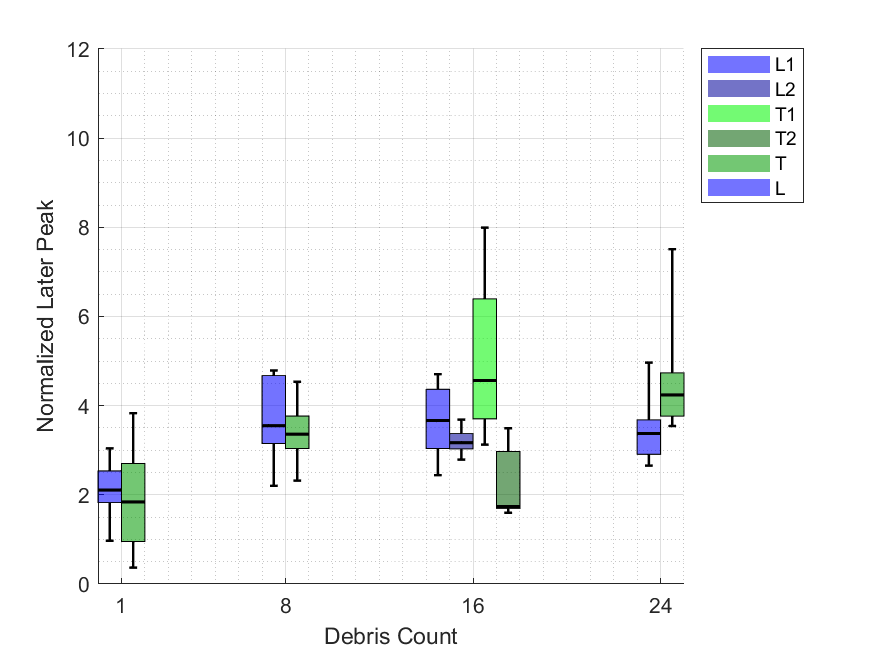
\includegraphics[width=0.8\textwidth]{LaterPeak_Regular_SplitByTrial.png}
    \caption{Later peak forces in regular arrangements (split by trial). Nonlinear growth and saturation effects evident.}
    \label{fig:laterpeak_regular_split}
\end{figure}

\begin{figure}[htbp]
    \centering
    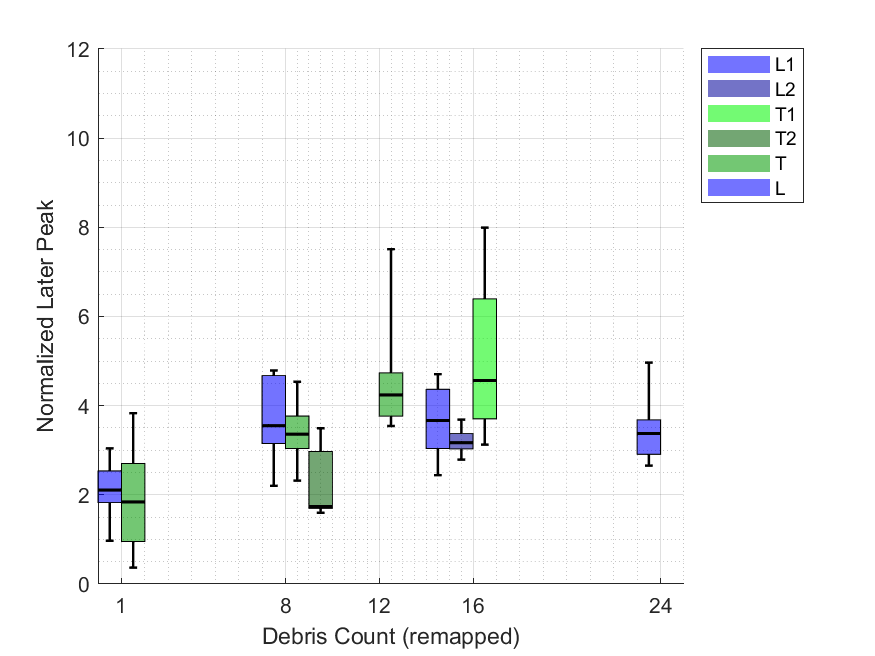
\includegraphics[width=0.8\textwidth]{LaterPeak_Regular_RemappedT.png}
    \caption{Later peak forces in regular arrangements (remapped to normalized time). Variability increases with debris spreading beyond structure width.}
    \label{fig:laterpeak_regular_remap}
\end{figure}

\subsection{Random Configurations}
\begin{itemize}
    \item Random debris fields produced more scattered and generally smaller peaks compared to regular arrangements.
    \item Multi-size fields consistently yielded lower impact magnitudes because smaller blocks contributed less momentum.
    \item The influence of \textbf{surface area density} was pronounced:
    \begin{itemize}
        \item At low density, debris was widely dispersed, lowering the chance of structural contact.
        \item At high density, debris filled the flume width, forcing many pieces away from the structure.
        \item Thus, for large debris groups at the same nominal density as smaller groups, the probability of impact decreased once the debris field spanned wider than the structure.
    \end{itemize}
\end{itemize}

\begin{figure}[htbp]
    \centering
    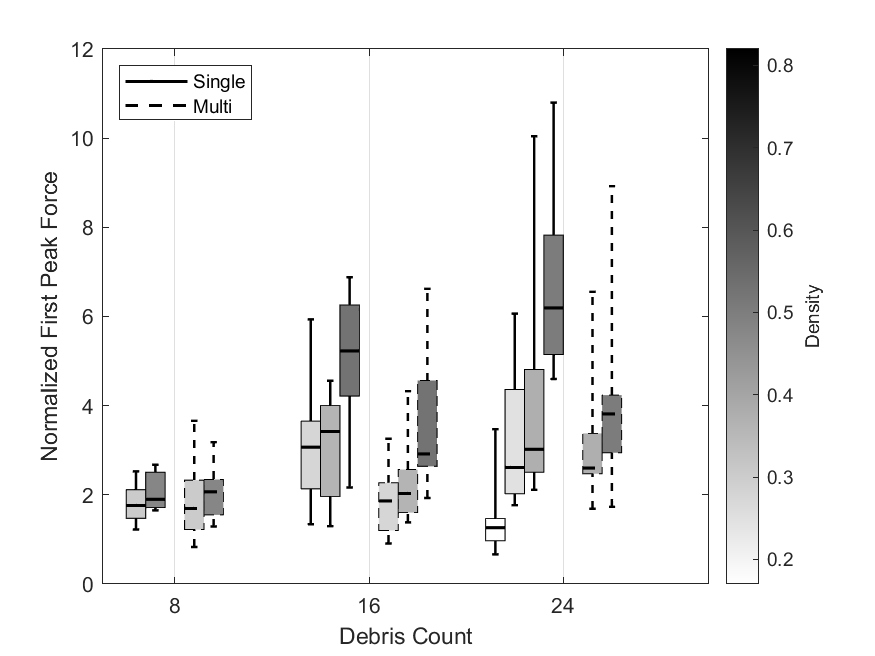
\includegraphics[width=0.8\textwidth]{First_Peak_Random_Single_vs_Multi_ByDensityGradient.png}
    \caption{First peak forces in random debris fields. Multi-size cases yield smaller peaks across surface area density gradients.}
    \label{fig:random_peaks_first}
\end{figure}

\begin{figure}[htbp]
    \centering
    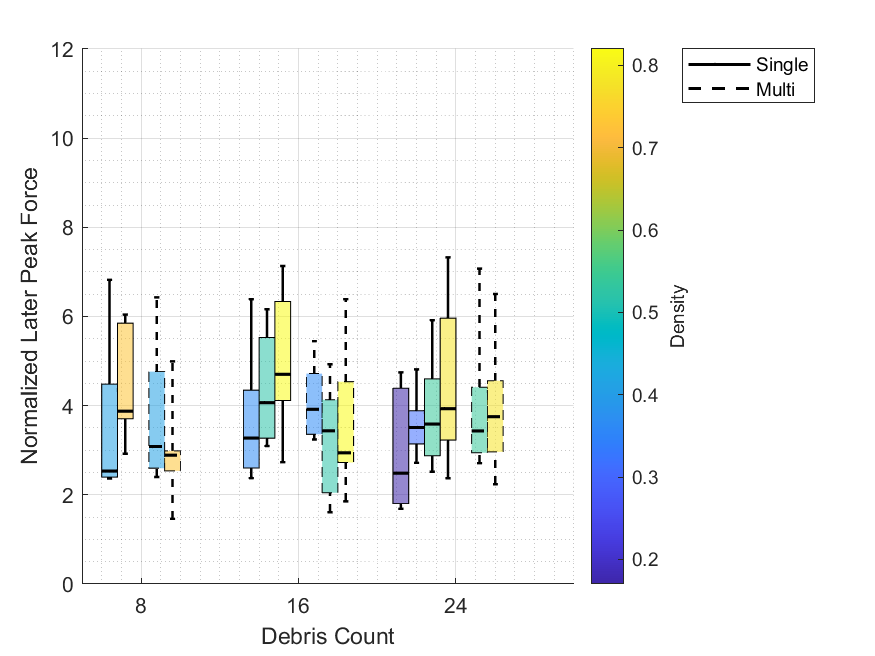
\includegraphics[width=0.8\textwidth]{LaterPeak_Random_Single_vs_Multi_ByDensityGradient.png}
    \caption{Later peak forces in random debris fields. Strong variability with density, with multi-size consistently lower.}
    \label{fig:random_peaks_later}
\end{figure}

\section{Results: Damming Forces (Unbroken Waves)}
\begin{itemize}
    \item Damming forces, extracted by low-pass filtering, reflected sustained blockage effects.
    \item \textbf{Single-size debris}: increasing surface area density led to stable jams and steadily increasing damming loads.
    \item \textbf{Multi-size debris}: smaller blocks prevented stable blockages, keeping damming forces consistently lower.
    \item Regular longitudinal and transverse cases produced comparable damming magnitudes, showing geometry was less critical than surface area density.
    \item Density had a pronounced effect for single-size debris but only weak influence for multi-size.
\end{itemize}

\begin{figure}[htbp]
    \centering
    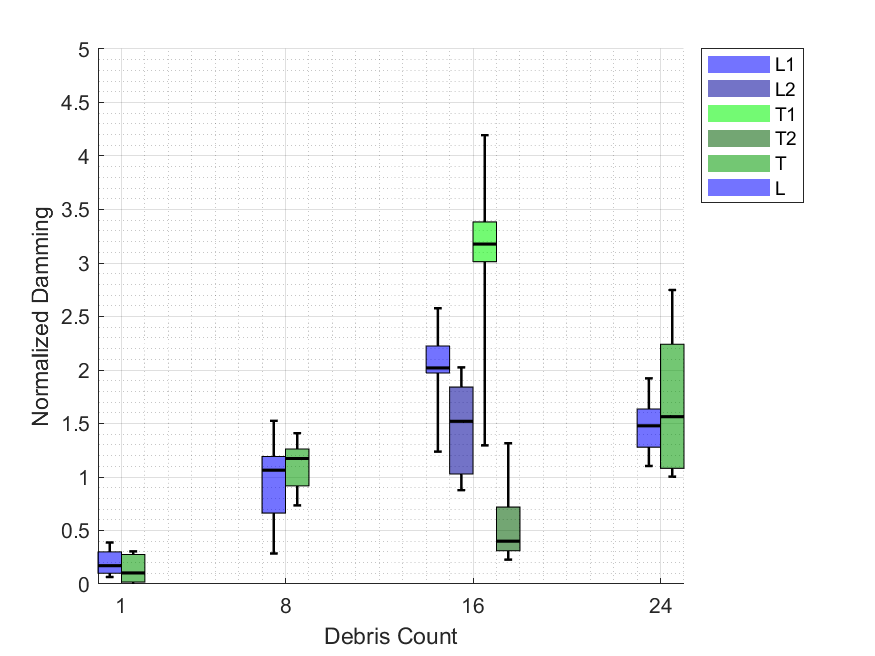
\includegraphics[width=0.8\textwidth]{Damming_Regular_L_T_SplitByTrial.png}
    \caption{Damming forces in regular arrangements (split by trial). Surface area density increases lead to higher sustained loads.}
    \label{fig:damming_regular_split}
\end{figure}

\begin{figure}[htbp]
    \centering
    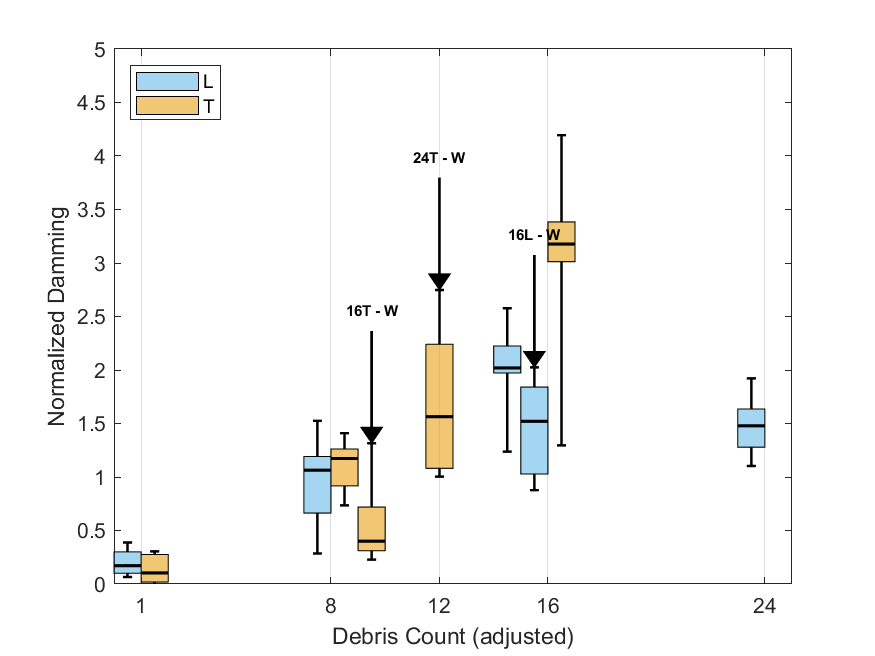
\includegraphics[width=0.8\textwidth]{Damming_Regular_L_T_SplitByTrial_Remapped.png}
    \caption{Damming forces in regular arrangements (remapped to normalized time). Consistent density effects across trials, with corrections applied to 24T and 16T2.}
    \label{fig:damming_regular_remap}
\end{figure}

\begin{figure}[htbp]
    \centering
    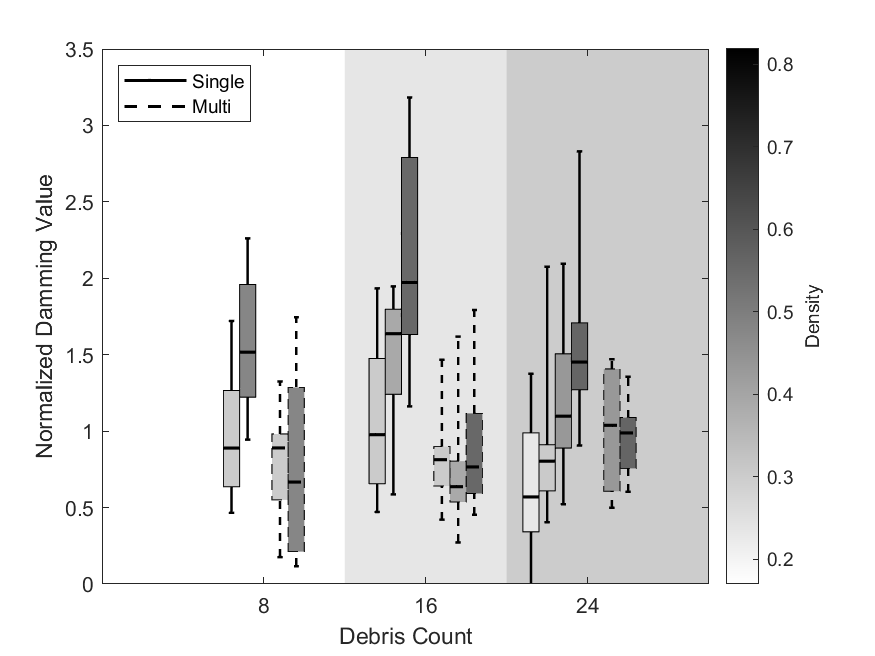
\includegraphics[width=0.8\textwidth]{Damming_Random_Single_vs_Multi_ByDensityGradient.png}
    \caption{Damming forces in random debris fields. Single-size cases develop strong jams; multi-size cases disrupted by small blocks.}
    \label{fig:damming_random}
\end{figure}

\section{Conclusions}
\begin{itemize}
    \item Longitudinal debris groups generated the largest impact peaks, while transverse groups were dominated by damming loads.
    \item Random and multi-size debris fields produced smaller and more variable forces due to reduced momentum transfer and disrupted blockage.
    \item \textbf{Surface area density effects:}
    \begin{itemize}
        \item Increasing debris count at fixed density forced the debris field to span more of the flume width.
        \item Once the debris spread exceeded the structure’s width, the probability of impact declined, leading to nonlinear or saturated growth of peak forces.
    \end{itemize}
    \item For 24T and 16T2 regular trials, debris spread exceeded the structure’s width. Video evidence confirmed partial impact, and data was corrected through remapping.
    \item First impacts scaled with debris count under aligned conditions, while later impacts were strongest in small groups and irregular in larger ones.
    \item Damming loads in multi-size fields were consistently weaker, highlighting the role of small blocks in preventing stable jams.
\end{itemize}

\section{References}
Bonus, J., Arduino, P., Motley, M., and Eberhard, M. (2022). ``Multi-Scale Numerical Simulation of Tsunami-Driven Debris-Field Impacts.'' In \textit{Ports 2022}, 328–39. https://doi.org/10.1061/9780784484395.033.

Derschum, C., Nistor, I., Stolle, J., and Goseberg, N. (2018). ``Debris Impact under Extreme Hydrodynamic Conditions Part 1: Hydrodynamics and Impact Geometry.'' \textit{Coastal Engineering}, 141: 24–35. https://doi.org/10.1016/j.coastaleng.2018.08.016.

Mascarenas, D., Motley, M. R., Eberhard, M. O., Arduino, P., and Serrone, A. (2022). ``Quantifying and Understanding Structural Loading from Wave-Driven Debris Fields.'' In \textit{Ports 2022}, 523–34. https://doi.org/10.1061/9780784484395.052.

Shekhar, K., Winter, A. O., Alam, M. S., Arduino, P., Miller, G. R., Motley, M. R., Eberhard, M. O., Barbosa, A. R., Lomonaco, P., and Cox, D. T. (2020). ``Conceptual evaluation of tsunami debris field damming and impact forces.'' \textit{Journal of Waterway, Port, Coastal, and Ocean Engineering}, 146(6), 04020039.

\end{document}
